\documentclass[10pt,a4paper]{article}

% ─── Packages ─────────────────────────────────────────

\usepackage{fontspec}
\setmainfont{Times New Roman}

\usepackage[top=0.9cm,bottom=0.9cm,left=1.5cm,right=1.5cm]{geometry}

\usepackage{titlesec}
\usepackage{enumitem}
\usepackage{hyperref}
\usepackage{xcolor}
\usepackage{tabularx}
\usepackage{graphicx}
\usepackage{parskip}

% ─── Colors ───────────────────────────────────────────

\definecolor{primary}{RGB}{30,40,90}
\definecolor{namecolor}{RGB}{0,120,180}
\definecolor{accent}{RGB}{50,90,150}
\definecolor{rulecol}{RGB}{200,205,220}
\definecolor{gray}{RGB}{90,90,90}

\hypersetup{
    colorlinks=true,
    urlcolor=accent
}

\pagestyle{empty}
\setlength{\parskip}{0pt}

% ─── Section ──────────────────────────────────────────

\titleformat{\section}
    {\normalsize\bfseries\color{primary}}
    {}
    {0em}
    {}
    [\vspace{1pt}\textcolor{rulecol}{\titlerule[0.6pt]}\vspace{1pt}]

\titlespacing{\section}{0pt}{3pt}{1pt}

% ─── Entry ────────────────────────────────────────────

\newcommand{\entry}[3]{%
    \noindent
    \begin{tabularx}{\linewidth}{X r}
        \textbf{\color{primary}#1} &
        {\scriptsize\color{gray}#2}
    \end{tabularx}\\[-2pt]
    {\scriptsize\textit{\color{gray}#3}}
    \vspace{1pt}
}

% ─── Compact list ─────────────────────────────────────

\newenvironment{cvitems}{
    \begin{itemize}[
        leftmargin=1.15em,
        topsep=0pt,
        itemsep=0.5pt,
        parsep=0pt,
        partopsep=0pt
    ]
}{
    \end{itemize}
}

% ═════════════════════════════════════════════════════

\begin{document}

% ─── HEADER ───────────────────────────────────────────

\noindent
\begin{tabularx}{\linewidth}{@{}X r@{}}

\begin{minipage}[c]{\linewidth}

    {\LARGE\bfseries\color{namecolor} Ho Huynh Nhu}\\[2pt]

    {\large\bfseries\color{primary}
    Software Tester (QA)}\\[3pt]

    {\scriptsize\color{gray}
    20/10/2003
    \enspace\textcolor{rulecol}{|}
    \enspace (+84) 367 503 477
    \enspace\textcolor{rulecol}{|}
    \enspace
    \href{mailto:hhnhu2003@gmail.com}{hhnhu2003@gmail.com}
    \enspace\textcolor{rulecol}{|}
    \enspace Ho Chi Minh City}\\[2pt]

    {\scriptsize
    \href{https://github.com/hohuynhnhu}
    {github.com/hohuynhnhu}
    \enspace\textcolor{rulecol}{|}
    \enspace
    \href{https://www.facebook.com/huynhnhu.ho.961}
    {facebook.com/huynhnhu.ho.961}
    }

\end{minipage}

&

\begin{minipage}[c]{2.2cm}
    \raggedleft
    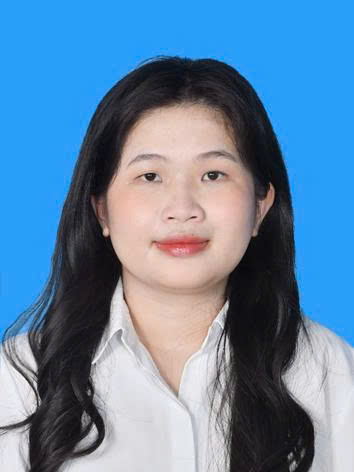
\includegraphics[
        width=2.2cm,
        height=2.7cm,
        keepaspectratio
    ]{assets/avt.jpg}
\end{minipage}

\end{tabularx}

\vspace{3pt}
\textcolor{rulecol}{\rule{\linewidth}{0.6pt}}

% ─── CAREER OBJECTIVE ─────────────────────────────────

\section*{Career Objective}

{\small
Final-year IT student with programming, SDLC, and database
fundamentals, plus hands-on practice testing AI/ML models and
FastAPI systems (test case design, functional/integration testing,
cross-validation, bug tracking). Upper-intermediate English,
strong passion for technology, and eager to build a solid QA
foundation through a mentorship-driven program such as NAB WeCamp.
}

% ─── EDUCATION ────────────────────────────────────────

\section*{Education}

\entry
{University of Transport Ho Chi Minh City (UTH)}
{10/2022 -- 10/2026}
{Bachelor of Information Technology -- Completed coursework}

{\small
\begin{cvitems}
    \item GPA: 3.4 / 4.0
    \item \textbf{Excellent Scholarship} -- Semester 1, 2025
    \item \textbf{Second Prize -- AI Track},
    UTH Student Scientific Research Conference 2025
\end{cvitems}
}

% ─── TESTING / TECHNICAL SKILLS ───────────────────────

\section*{Technical Skills}

{\small
\begin{tabularx}{\linewidth}{@{}lX@{}}

\textbf{AI / Model Testing}
&
Model Evaluation, Accuracy/Precision/Recall/F1 Analysis,
K-Fold Cross-Validation, Error Analysis, Regression Testing
of Model Versions
\\[1.5pt]

\textbf{Functional \& API Testing}
&
Manual Testing, Test Case Design, API Testing (Postman),
Integration Testing, End-to-End Testing of FastAPI Services
\\[1.5pt]

\textbf{Computer Vision \& AI Dev}
&
Object Detection, Pose Estimation, Face Recognition, MediaPipe;
built with Python, PyTorch, OpenCV, Ultralytics YOLO, FastAPI
\\[1.5pt]

\textbf{Data \& Reporting}
&
PostgreSQL, SQL Server, MongoDB, Firebase, Supabase,
dbt, Airflow, Power BI
\\[1.5pt]

\textbf{Tools}
&
Git, Docker, Postman, VS Code, Jira/bug tracking, Power BI
\\[1.5pt]

\textbf{Programming}
&
Python, SQL, TypeScript, JavaScript, Kotlin
\\[1.5pt]

\textbf{English}
&
Upper-Intermediate -- clear written and spoken communication for
technical/professional contexts

\end{tabularx}
}

% ─── WORK EXPERIENCE ──────────────────────────────────

\section*{Work Experience}

\entry
{Gotik Consulting -- Data Engineer}
{Python \textbar{} dbt \textbar{} PostgreSQL \textbar{} Airflow}
{03/2026 -- 05/2026}

{\small
\begin{cvitems}
    \item Validated and reconciled Odoo data outputs against
    source records; developed and tested Python pipelines with
    dbt and Neon PostgreSQL, including data-quality checks.
    \item Monitored and verified automated Airflow workflows,
    investigating and resolving failed runs; built Power BI
    dashboards to cross-check operational metrics.
\end{cvitems}
}

% ─── PROJECTS ─────────────────────────────────────────
\section*{Featured AI Testing / Evaluation Projects}

\entry
{Fall Detection -- Real-Time AI Fall Detection System}
{Python \textbar{} YOLOv8 Pose \textbar{} MediaPipe \textbar{} Transformer \textbar{} FastAPI}
{04/2026 -- 06/2026}

{\small
\begin{cvitems}
    \item Designed and executed the evaluation plan for a real-time
    fall detection model (YOLOv8 Pose + MediaPipe + Transformer),
    covering offline model testing and live system testing.
    \item Ran 5-fold cross-validation (Transformer Encoder, 30-frame
    $\times$ 200-feature input), achieving 97.8\% mean accuracy.
    \item Tested the FastAPI real-time alert pipeline end-to-end
    to confirm detection latency and correctness.
    \item GitHub: \href{https://github.com/hohuynhnhu/Fall-Detection}{Fall-Detection}
\end{cvitems}
}

\vspace{1pt}

\entry
{VehicleScan -- Smart Parking System with AI \& IoT}
{Python \textbar{} YOLO \textbar{} CNN \textbar{} Siamese Network \textbar{} ESP32}
{03/2025 -- 03/2026}

{\small
\begin{cvitems}
    \item Tested vehicle detection/recognition models (YOLO, CNN,
    Siamese Network) against labeled datasets to measure and
    improve recognition accuracy.
    \item Performed integration testing between AI models, ESP32
    hardware, and Firebase; reported and helped fix edge-case
    failures. Won Second Prize -- AI Track, UTH 2025.
    \item GitHub: \href{https://github.com/LeKhang-cn22h/VehicleScanner.git}{VehicleScanner}
\end{cvitems}
}

% ─── ADDITIONAL INFORMATION ───────────────────────────

\section*{Additional Information}

{\small
\begin{tabularx}{\linewidth}{@{}lX@{}}

\textbf{Soft Skills}
&
Attention to detail \textbar{}
Analytical / root-cause thinking \textbar{}
Teamwork \textbar{}
Troubleshooting
\\[2pt]

\textbf{QA Interests}
&
AI/ML Model Evaluation \textbar{}
API \& System Testing \textbar{}
Test Automation \textbar{}
QA for Real-time Systems
\\[2pt]

\textbf{Availability}
&
Final-year student / career switcher into QA -- available to join
NAB WeCamp full-time.

\end{tabularx}
}

\end{document}